\documentclass{beamer}

\input{../Haust2015glærur}

\title{Tölvunarfræði 1a}
\subtitle{Vika 4, fyrri fyrirlestur}

\begin{document}

\begin{frame}
\titlepage
\end{frame}

\section{Inngangur}


\begin{frame}{Í síðasta þætti\ldots}
\begin{itemize}
 \item Inntak og úttak
 \begin{itemize}
  \item \texttt{input}
  \item \texttt{fprintf}
 \end{itemize}
 \item Einfaldar myndir
 \begin{itemize}
  \item \texttt{plot}
 \end{itemize}
 \item Einföld skráarnotkun
 \begin{itemize}
  \item \texttt{save} og \texttt{load}
 \end{itemize}
\end{itemize}
Kaflar: 3.3 til 3.6
\end{frame}

\begin{frame}{Gömul fyrirlestrarræfing}
\begin{itemize}
 \item Skrifið skipanaskrá sem biður notanda um nafn og skrifar út lengd nafnsins (fallið \texttt{length})
\end{itemize}
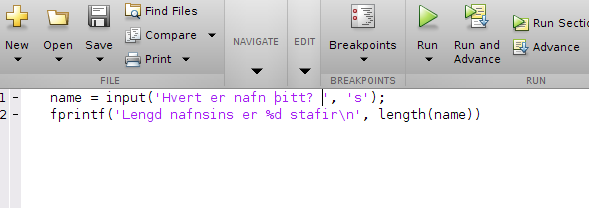
\includegraphics[width=\textwidth]{Pics/name-length}
\end{frame}

\begin{frame}{Gömul fyrirlestraræfing}
\begin{columns}
\column{0.6\textwidth}
\begin{enumerate}
\setcounter{enumi}{2}
 \item Hér til hliðar eru hitamælingar fyrir septemberdag í Reykjavík. Sýnið snyrtilegt línurit fyrir hitastigið þennan dag.
 \item Vistið þessar upplýsingar í skrá.
\end{enumerate}
\column{0.4\textwidth}
\begin{center}
\begin{tabular}{ll}
\toprule
Klst&$C^\circ$\\
\midrule
0&12.5\\
3&12.4\\
6&12.3\\
9&12.8\\
12&13.4\\
15&14\\
18&13.1\\
21&12.8\\
\bottomrule
\end{tabular}
\end{center}
\end{columns}
\end{frame}

\begin{frame}[fragile]{Gömul fyrirlestrarræfing}
\begin{center}
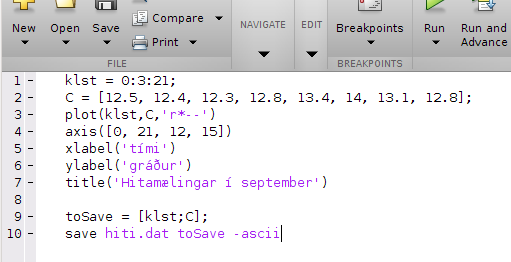
\includegraphics[width=0.9\textwidth]{Pics/septemberhitiscript}
\end{center}
\end{frame}

\begin{frame}[fragile]{Gömul fyrirlestrarræfing}
\begin{center}
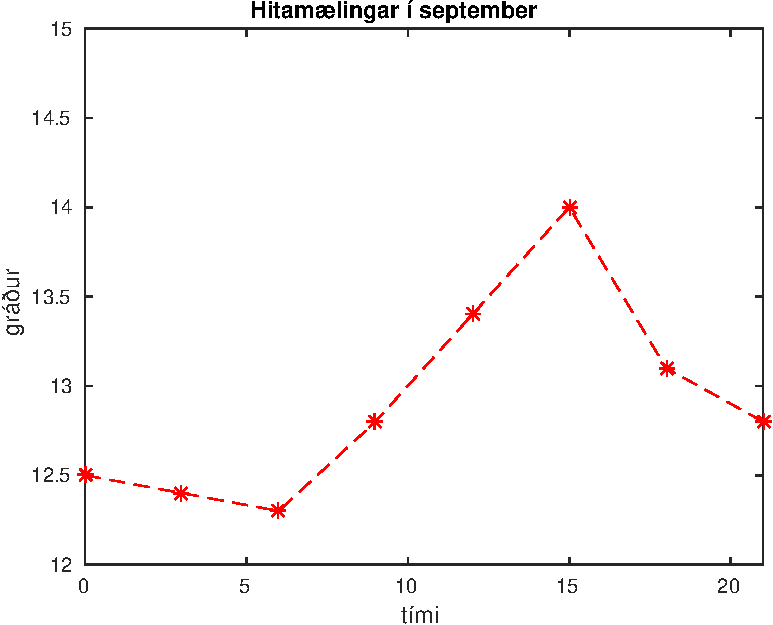
\includegraphics[width=0.7\textwidth]{Pics/septemberhiti}
\end{center}
\end{frame}

\section{Föll (3.7)}

\begin{frame}{Upprifjun á fallshugtakinu}
\begin{itemize}
 \item Föll eru notuð til að framkvæma ákveðna útreikninga sem \emph{byggja á inntaksgildum}
 \begin{itemize}
  \item Föllin taka inn gildi, reikna með gildunum, og skila niðurstöðu.
  \item Oftast er útkoman eitt gildi, niðurstaða útreikninga
 \end{itemize}
\end{itemize}
\end{frame}

\begin{frame}[fragile]{Dæmi}
Dæmi: Fallið \texttt{distance}, sett í skrána \texttt{distance.m}.
\begin{minted}[frame=lines]{matlab}
function d = distance(v, t)
  d = v*t;
end  
\end{minted}
Þetta fall heitir \texttt{distance}, tekur inn breytu $v$ sem táknar (meðal)hraða, lengd tímabils $t$ og skilar fjarlægð. Eftir að það hefur verið skilgreint má nota það alls staðar í sömu möppu (í skipanaglugga, í skipanaskrám, í öðrum föllum).
\end{frame}

\begin{frame}{Föll vs. skipanaskrár}
\begin{itemize}
 \item \emph{Mjög auðvelt} er að rugla saman hugtökunum um föll og skipanaskrár
 \begin{itemize}
  \item Hvort tveggja er geymt í skrá
 \end{itemize}
 \item Fall er safn af skipunum sem táknar ákveðna gerð af útreikningum
 \begin{itemize}
  \item Fyrsta orðið er \texttt{function}
  \item Inntök og úttök skilgreind í haus fallsins
 \end{itemize}
 \item Skipanaskrá er samansafn af hvaða Matlab-skipunum sem er
 \begin{itemize}
  \item Venjulega er inntak skilgreint með \texttt{input} og útskrift með \texttt{disp} eða \texttt{fprintf}
  \item Skipanaskrá \emph{skilar} ekki gildi!
 \end{itemize}
\end{itemize}
\end{frame}

\begin{frame}{Föll og skipanaskrár eru vinir}
Algengt mynstur:
\begin{itemize}
 \item Skipanaskrár lesa inntak og skrifa úttakið
 \item Föll framkvæma útreikninga
\end{itemize}

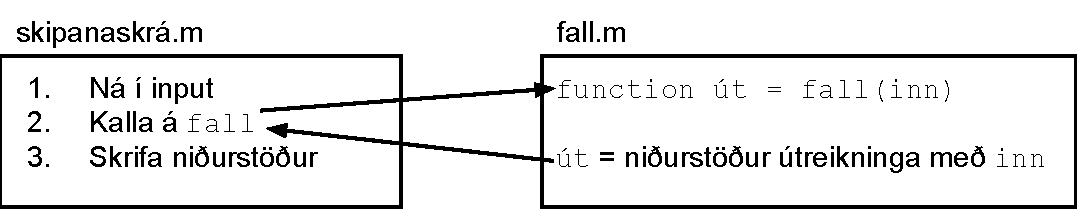
\includegraphics[width=\textwidth]{Pics/skripta-og-fall}
\end{frame}

\begin{frame}{Dæmi: Síðasta tímaverkefni}
\begin{center}
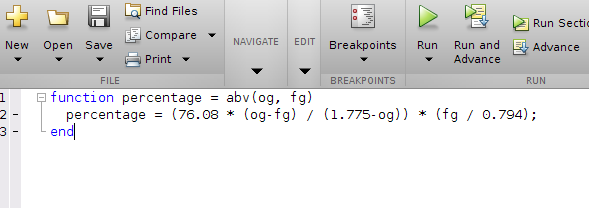
\includegraphics[width=\textwidth]{Pics/abv-function}\\
\vspace{\baselineskip}
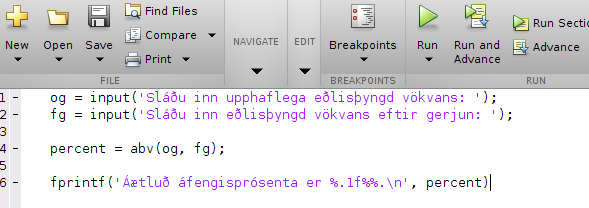
\includegraphics[width=\textwidth]{Pics/abv-script}
\end{center}
\end{frame}

\begin{frame}[fragile]{Hagnýt atriði}
\begin{itemize}
 \item Hafið hvert fall eitt og sér í skrá
 \begin{itemize}
  \item Nefnið skrána sama nafni og fallið, nema skráin hefur endinguna \texttt{.m}
 \end{itemize}
 \item Breyturnar og geta verið með jafn fjölskrúðug nöfn og aðrar breytur í Matlab
 \item Ekki nefna breytur og skipanaskrár sama heiti
\end{itemize}
\end{frame}

\begin{frame}[fragile]{Forritunarvenjur}
\begin{columns}
\column{0.5\textwidth}
\begin{itemize}
 \item Algengt: Skjölun (e. \emph{documentation}), þ.e.a.s. staðlaðar athugasemdir efst í falli
 \begin{itemize}
  \item Lýsing á því hvað fallið gerir
  \item Hvernig á að kalla á fallið
  \item Form inntaksbreyta (stika)
  \item Form skilagildis
  \item Breytingasaga
 \end{itemize}
 \item Inndráttur
 \begin{itemize}
  \item Smart Indent (ctrl+i) í Matlab ritli gerir þetta fyrir okkur
 \end{itemize}
\end{itemize}
\column{0.5\textwidth}
\begin{minted}[frame=lines]{matlab}
function c = fahrToCelc(f)
% fahrToCelc breytir úr F í C
% Notkun:  fahrToCelc(fhiti)
   c = (f-32)*5/9;
end
\end{minted}

\end{columns}
\end{frame}

\subsection{Staðværar breytur}

\begin{frame}{Staðværar breytur}
\begin{itemize}
 \item Stundum þarf að skilgreina nýjar breytur inni í föllum
 \begin{itemize}
  \item Þær eru þá staðværar (e. \emph{local}) innan fallsins
  \item Þær hverfa úr minninu þegar fallið hefur lokið keyrslu
  \item Valda ekki árekstrum við aðrar breytur utan fallsins
 \end{itemize}
\end{itemize}
\end{frame}

\begin{frame}{Framkvæmd}
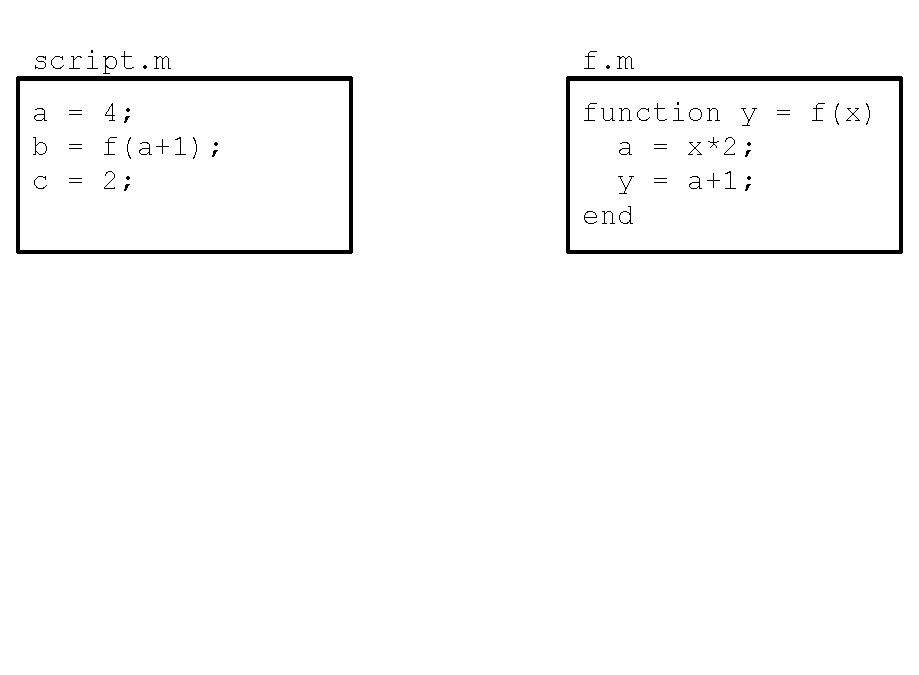
\includegraphics[width=\textwidth]{Pics/framkvaemd-falls-0}
\end{frame}
\begin{frame}{Framkvæmd}
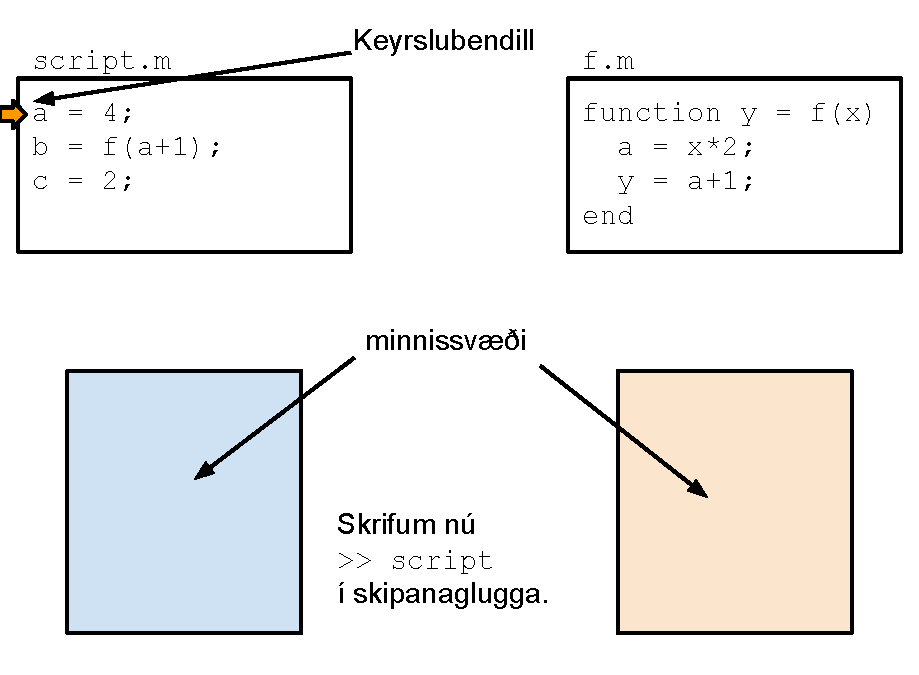
\includegraphics[width=\textwidth]{Pics/framkvaemd-falls-1}
\end{frame}
\begin{frame}{Framkvæmd}
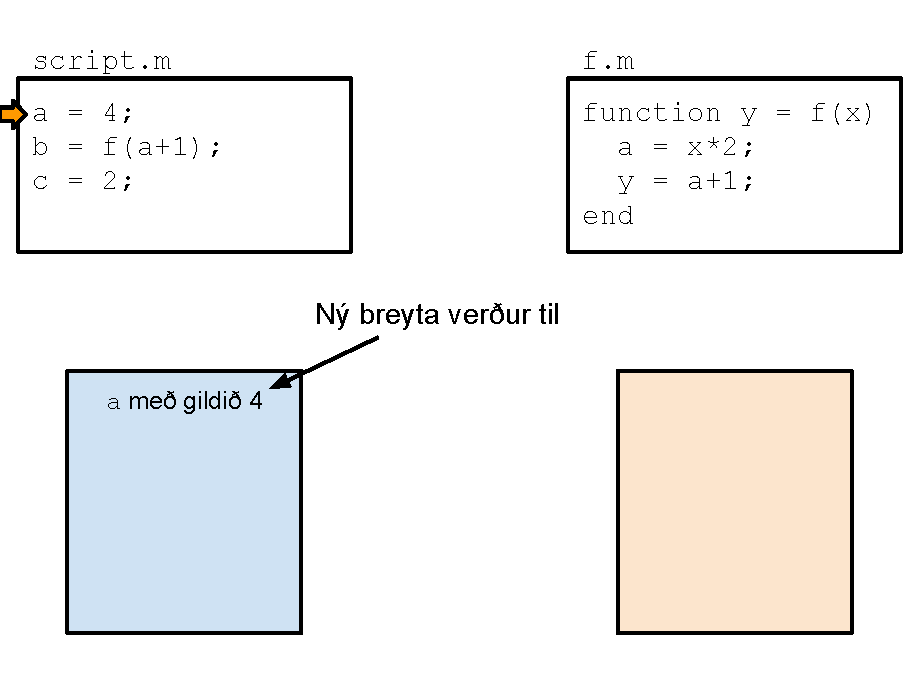
\includegraphics[width=\textwidth]{Pics/framkvaemd-falls-2}
\end{frame}
\begin{frame}{Framkvæmd}
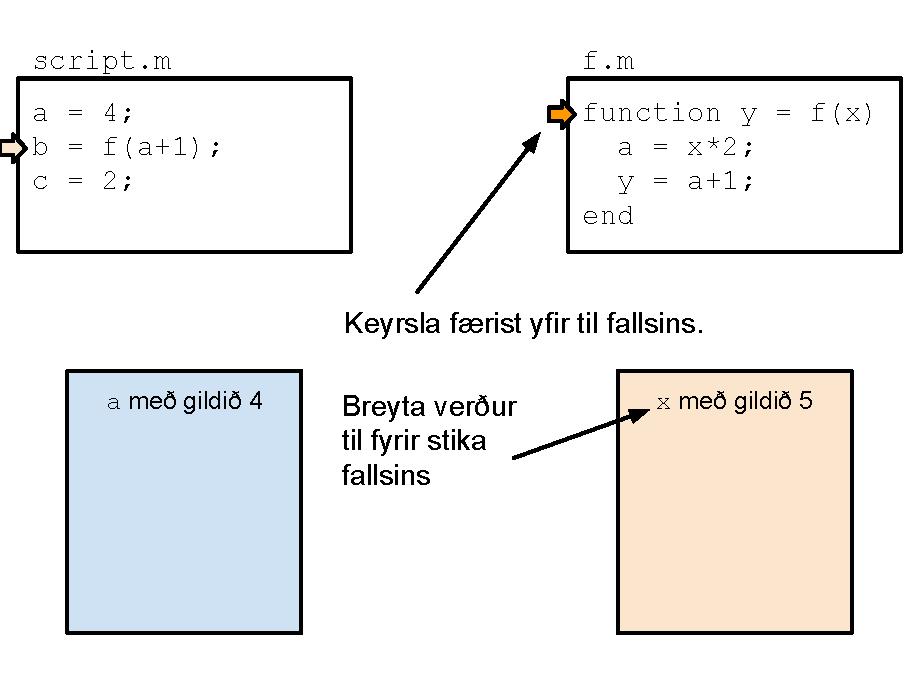
\includegraphics[width=\textwidth]{Pics/framkvaemd-falls-3}
\end{frame}
\begin{frame}{Framkvæmd}
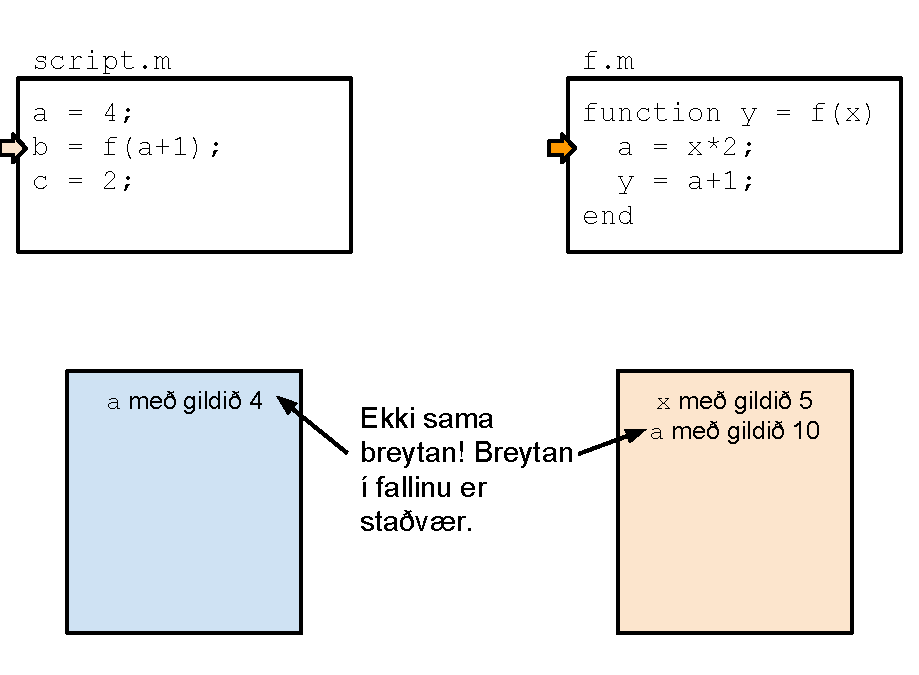
\includegraphics[width=\textwidth]{Pics/framkvaemd-falls-4}
\end{frame}
\begin{frame}{Framkvæmd}
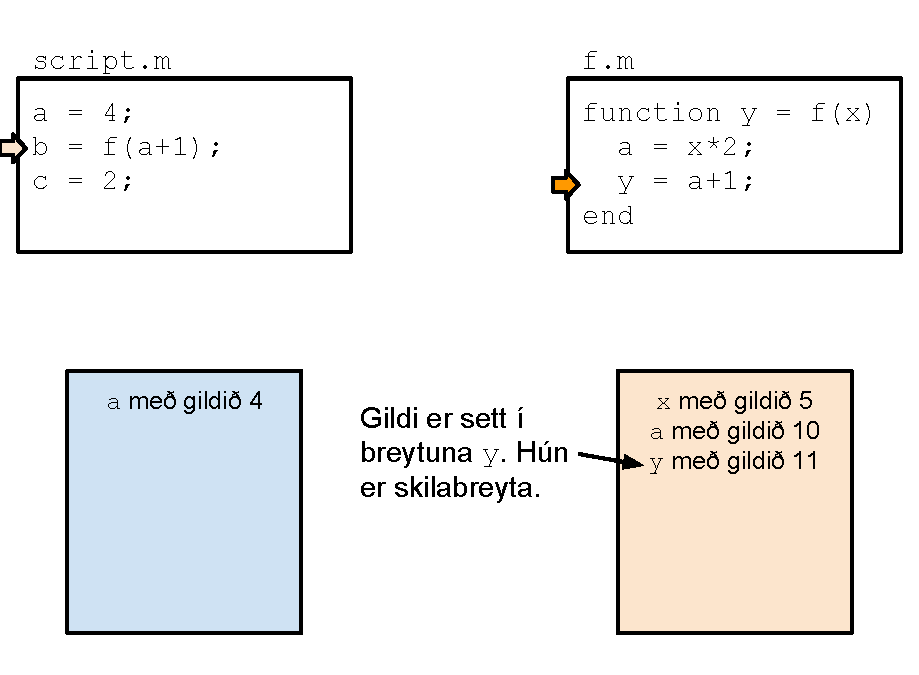
\includegraphics[width=\textwidth]{Pics/framkvaemd-falls-5}
\end{frame}
\begin{frame}{Framkvæmd}
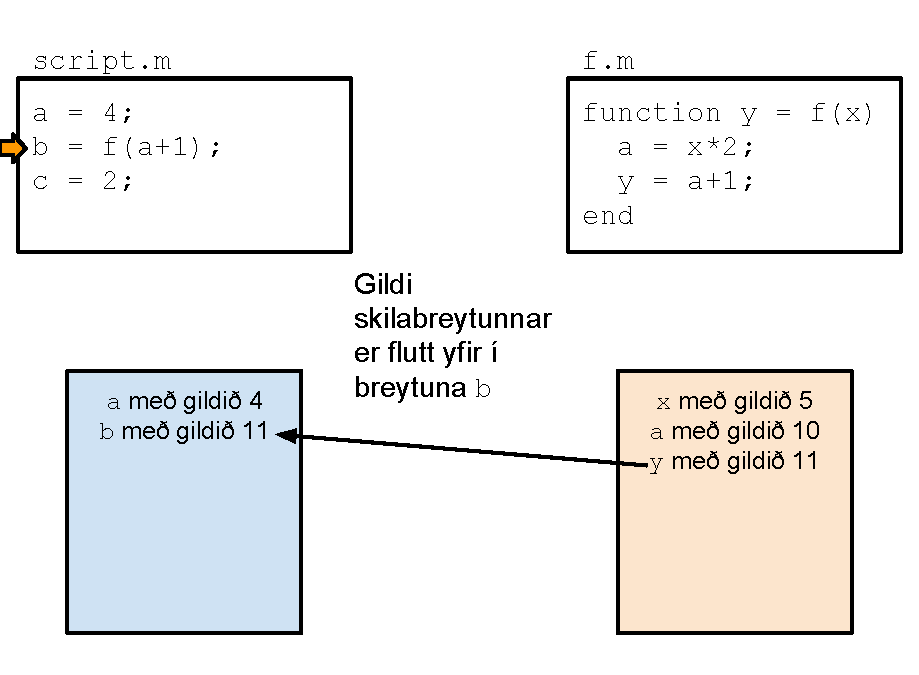
\includegraphics[width=\textwidth]{Pics/framkvaemd-falls-6}
\end{frame}
\begin{frame}{Framkvæmd}
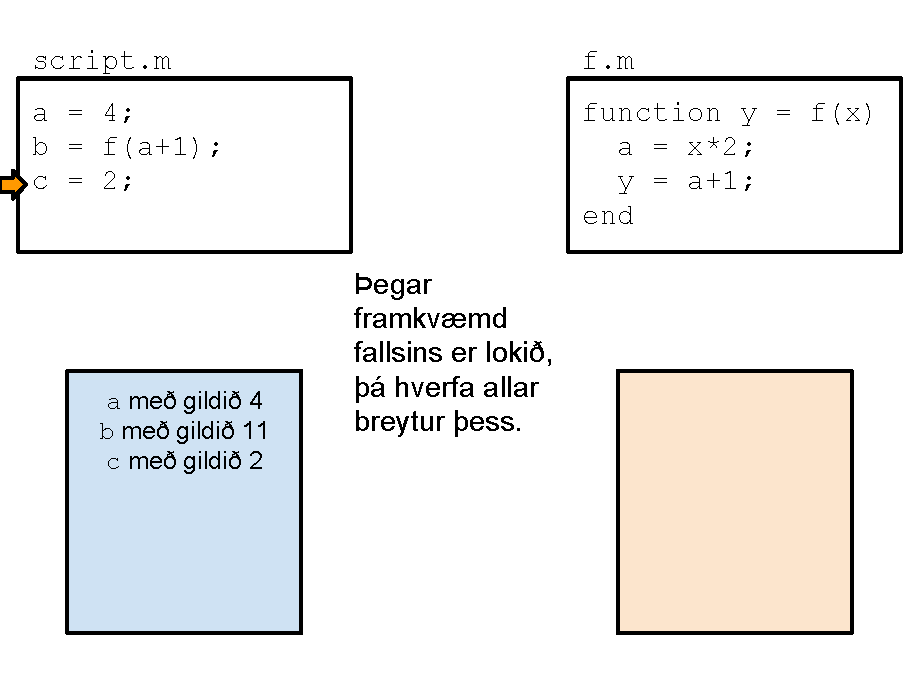
\includegraphics[width=\textwidth]{Pics/framkvaemd-falls-7}
\end{frame}

\begin{frame}{fyrirlestrarræfing}
\begin{enumerate}
 \item Skrifið fallið \texttt{celcToFahr}, sem breytir Celsíus hitastigi yfir í Fahrenheit ($f = c\cdot1.8 + 32$)
 \item Skilgreinið breytuna $z$ í skipanaglugganum. Skilgreinið líka fallið $fz$. Getur notendaskilgreinda fallið $fz$ notað breytuna z úr skipanaglugganum? Getur skipanaskrá gert það?
\end{enumerate}
\end{frame}

\section{Stýrisetningar}

\subsection{if (4.1)}

\begin{frame}{Stýrisetningin if}
\begin{columns}
\column{0.5\textwidth}
\begin{itemize}
 \item Hingað til hefur því verið haldið fram að hver einasta lína í falli eða skipanaskrá sé keyrð á eftir þeirri sem er fyrir ofan \pause
 \begin{itemize}
  \item \ldots það er lygi. \pause
 \end{itemize}
 \item Skipun til að velja hvort að ``blokk'' af kóða sé keyrð eða ekki er \texttt{if}-skipun
\end{itemize}
\column{0.5\textwidth}
\begin{center}
 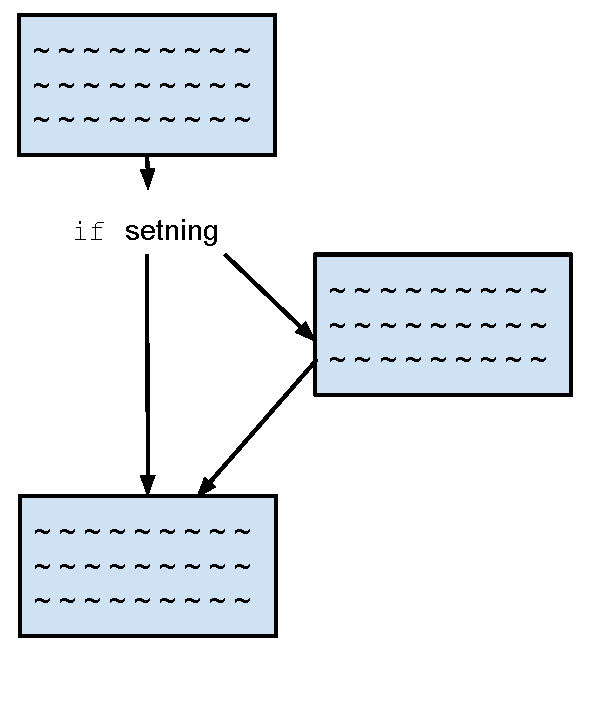
\includegraphics[width=0.8\linewidth]{Pics/if}
\end{center}
\end{columns}
\end{frame}

\begin{frame}[fragile]{Uppbygging if-skipunar}
\vspace{\baselineskip}
Hér eru skipanirnar einungis framkvæmdar ef ákveðið \emph{skilyrði} er uppfyllt.

\begin{verbatim}
if skilyrði
  skipun
  skipun
  ...
  skipun
end
\end{verbatim} 
Þetta skilyrði er \emph{rökyrðing} sem í einhverjum skilningi er sönn eða ósönn.

\end{frame}

\begin{frame}{Upprifjun - rökyrðingar}
\begin{itemize}
 \item Rökyrðingar (e. \emph{logical expressions}) vinna með \emph{sanngildi} í stað talna.
 \begin{itemize}
  \item Sanngildi eru tvö: \texttt{true} og ósatt \texttt{false}
  \item Í Matlab er oft notað $1$ og $0$ í stað \texttt{true} og \texttt{false}
 \end{itemize}
 \item Notum samanburðarvirkja (e. \emph{relational operators}) og rökvirkja (e. \emph{logical operators})
\end{itemize}
\end{frame}

\begin{frame}{Upprifjun - samanburðarvirkjar}
\begin{columns}
\column{0.5\textwidth}
\begin{itemize}
 \item Samanburðarvirkjar bera saman gildi og skila sanngildi (e. \emph{truth value}).
 \item Sanngildi hafa sitt eigið tag, \texttt{logical}
\end{itemize}
\column{0.5\textwidth}

\vspace{0.5cm}
Samanburðarvirkjar í Matlab: 

\vspace{0.2cm}
\begin{tabular}{ll}
\toprule
Virki&Merking\\
\midrule
\texttt{>}&stærri en\\
\texttt{<}&minni en\\
\texttt{>=}&stærri en eða jafn ($\geq$)\\
\texttt{<=}&minni en eða jafn ($\leq$)\\
\texttt{==}&jafnt og\\
\texttt{\~}\texttt{=}&ekki jafnt og\\
\bottomrule
\end{tabular}
\end{columns}
\end{frame}

\begin{frame}{Upprifjun - rökvirkjar}
Rökvirkjar vinna með sanngildi:
\begin{center}
\begin{tabular}{ll}
\toprule
Virki&Merking\\
\midrule
||& eða, skilar satt ef annað viðfangið er satt\\
\&\& & og, skilar satt ef bæði viðföngin eru sönn\\
\~{} &ekki, skilar öfugu við viðfangið\\
\bottomrule
\end{tabular}
\end{center}
Einnig er til rökfallið \texttt{xor}. Það tekur tvö viðföng og skilar ``annaðhvort eða''. Satt ef annað viðfangið er satt, en ekki ef bæði eru sönn.
\end{frame}

\begin{frame}[fragile]{Dæmi um if-setningar}
Hér: Notað til að athuga hvort að gildi séu í lagi
\begin{minted}[frame=lines]{matlab}
if x >= 0
    fprintf('Kvaðratrót %f er %f\n', x, sqrt(x));
end
\end{minted}

\begin{minted}[frame=lines]{matlab}
if q ~= 0
    fx = (4*d + h)/q;
end
\end{minted}

\end{frame}

\begin{frame}[fragile]{Stærra dæmi}
Þetta mætti setja í skipanaskrá og keyra:
\begin{minted}[frame=lines]{matlab}
% Biðja notanda um tölu og prenta út kvaðratrót hennar
num = input('Sláið inn tölu: ');

% Ef talan er neikvæð, þá breyta henni
if num < 0
    num = 0;
end
fprintf('Kvaðratrót %.1f er %.1f\n', num, sqrt(num));
\end{minted}
\end{frame}

\begin{frame}[fragile]{Skilyrði í if-setningu}
Athugið að Matlab reynir að túlka hvað svosem sett er í skilyrðishluta \texttt{if}-setningar sem rökgildi.

\begin{minted}[frame=lines]{matlab}
>> if -4
disp('Já, þetta er satt')
end
Já, þetta er satt
\end{minted}
Ath: Slæm hugmynd að notfæra sér þetta viljandi.
\end{frame}

\begin{frame}{Algeng villa}
\begin{itemize}
 \item Gerum ráð fyrir að notandi hafi verið að segja okkur hvort forrit eigi að halda áfram
 \begin{itemize}
  \item \texttt{svar = input('Halda áfram (J/N): ','s');}
 \end{itemize}
 \item Vitum ekki hvort notandinn sagði \texttt{'j'} eða \texttt{'J'}, svo við athugum hvort tveggja
 \begin{itemize}
  \item \texttt{if svar == 'J' || 'j'}
  \item Hvað er að þessu? \pause
 \end{itemize}
 \item Bókstafirnir eru túlkaðir sem tölur (sem eru ekki núll), svo þetta verður alltaf satt!
 \item Rétt útgáfa: \texttt{if svar == 'J' || svar == 'j'}
\end{itemize}
\end{frame}

\subsection{if og else (4.2)}

\begin{frame}[fragile]{if-else setningin}
\begin{columns}
\column{0.5\textwidth}
Getum valið á milli tveggja hópa af setningum með \texttt{if-else} setningunni
\begin{verbatim}
if skilyrði
    setningar
else
    aðrar setningar
end
\end{verbatim}
Ef skilyrðið er satt þá er fyrri setningahópurinn framkvæmdur, annars seinni
\column{0.5\textwidth}
\begin{center}
 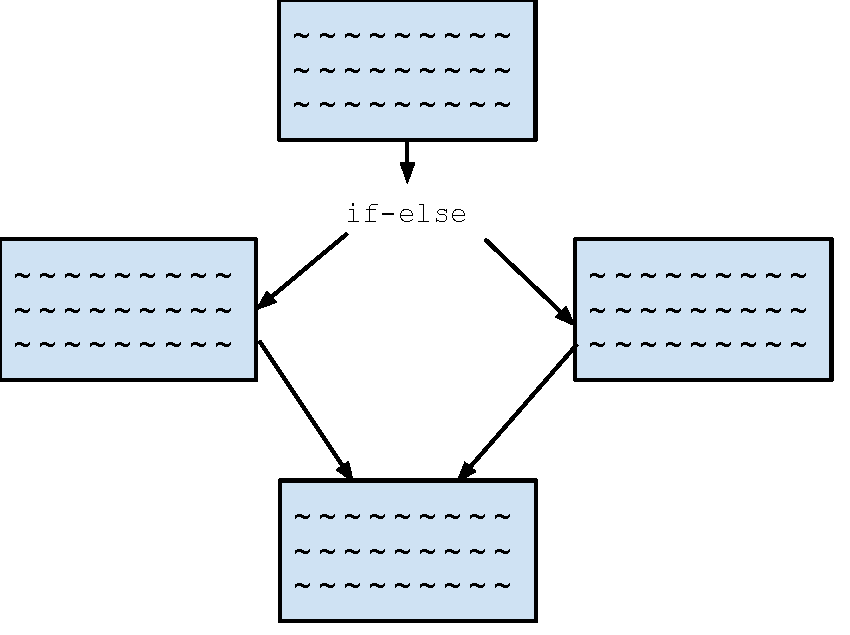
\includegraphics[width=\linewidth]{Pics/if-else}
\end{center}
\end{columns}
\end{frame}

\begin{frame}[fragile]{Dæmi um if-else setningar}
\begin{minted}[frame=lines]{matlab}
if rand() < 0.5
    disp('Þorskur');
else
    disp('Skjaldarmerki');
end
\end{minted}

\begin{minted}[frame=lines]{matlab}
rad = input('Sláðu inn radíus: ');
if rad < 0
    fprintf('%.2f er ólöglegur radíus\n', rad);
else
    area = pi * rad*rad;
    fprintf('Flatarmálið er %.2f\n', area);
end
\end{minted}
\end{frame}

\begin{frame}[fragile]{Útreikningur á skilyrði í if-setningu}
Skilyrði í \textbf{if}-setningu er aðeins reiknað út þar til útkoma þess er ljós, en ekki lengra.

\begin{minted}[frame=single]{matlab}
if (b ~= 0) && (a/b < 10.0)
    disp('Yes!');
end
\end{minted}
Ef \texttt{b} er 0 er seinni hluti skilyrðisins ekki reiknaður.

\end{frame}

\begin{frame}{fyrirlestrarræfing}
\begin{enumerate}
\setcounter{enumi}{2}
 \item Skrifið \texttt{if}-setningu sem prentar út villuskilaboð ef breytan \texttt{x} er minni en 0
 \item Skrifið \texttt{if}-setningu sem skrifar út hvort nemandi hafi fallið í námskeiði eða ekki (tvö mismunandi skilaboð).  Nemandi fellur ef prófeinkunn (\texttt{profeinkunn}) er lægri en 5.0
\end{enumerate}

\end{frame}


\end{document}
